\documentclass[../../master_thesis_np.tex]{subfiles}
\graphicspath{{./imgs/}}

\begin{document}
\chapter[Interaction Implementation]{Implementation of interactions in simulations}
\label{chap:int_impl}
	\section{Model}
	There are several examples in literature of aligning interactions applied to ABPs systems. Most of them involve applying a torque which explicitly depends on the difference between the orientation angle of the two interacting particles; some of them have a constant torque which is applied to particles closer than a certain distance. To the best of our knowledge, nobody tried before to implement an interaction in the system which unifies the central force and the torque. 
	
	The model used in this thesis aims to keep a minimal amount of parameters while coupling positions and orientations of interacting particles, actually using only one more parameter than a force-only model.
	
	If one was to apply a central force to a set of particles, the way would be computing a distance matrix between the positions of particles' centers, calculating the absolute value of the force with a function $F(r)$, and applying it to particle positions, splitting the two components (we are simulating in 2D).
	
	Here every particle is identified by two positions: its center of mass, which lies in its geometric center, and an interaction center, which is translated with respect to the center of mass of an amount $\alpha R$ in the direction of self-propulsion, so that the off center position of each particle writes:
	\begin{equation}
		\vec{x}_{oc} = \vec{x}_{cm} + \alpha R 
		\begin{pmatrix}
			\cos(\theta)\\
			\sin(\theta)
		\end{pmatrix}
	\end{equation}
	where $\theta$ is the self-propulsion direction, $R$ is the particle's radius, and $-1 < \alpha < 1$. This way distances, and hence forces, are computed starting from off center positions; applying forces to such positions results both in a translation effect and in a torque applied to the particle, coupling the two degrees of freedom.
	
	The idea is to take into account the underlying particle's asymmetry in simulations. It is a fact that the two faces of a Janus particle have different physical and chemical properties, which make them interact differently depending on the angle between their orientations and the line connecting their centers \cite{singh_pair_2024}. This can be due to a plethora of effects like chemical gradients, electrical forces or hydrodynamics, but this model takes only the asymmetry and uses it along with standard potentials, to create a minimal dry framework that mimics wet dynamics. In doing so, we also show that this model displays some interesting statistical mechanics properties.
	
	\begin{figure}[htp]
		\centering
		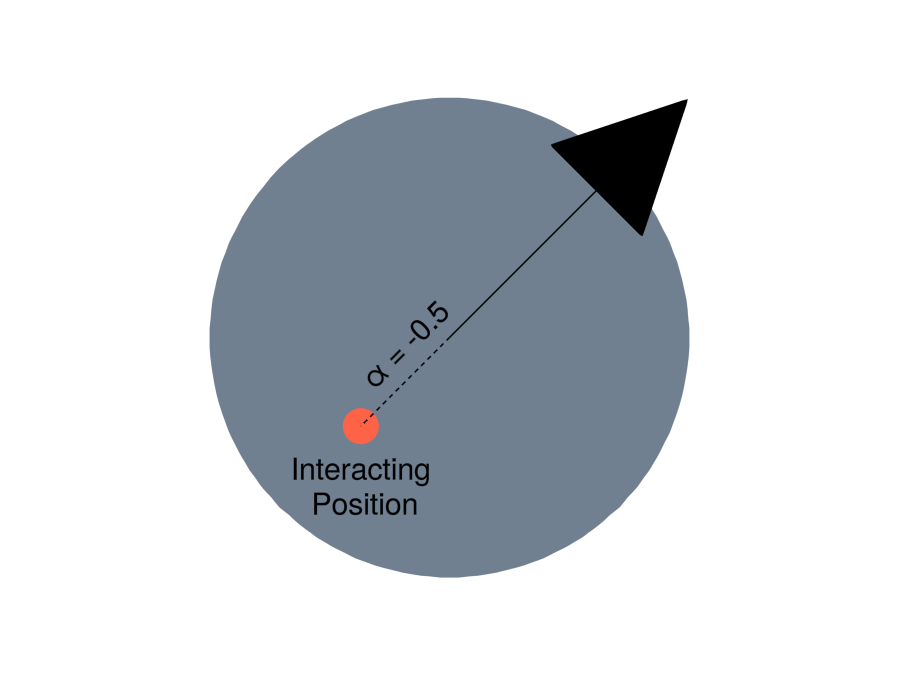
\includegraphics[width=\textwidth]{singpart_draw.png}
		\caption{}
		\label{fig:geom_model}
	\end{figure}
	
	\section{Methods}
	All the simulation and analysis code for this thesis was written in \julia, except for the machine learning and inference part, where the Graph Network definition and training makes use of Python libraries like PyTorch and PyTorch-geometric, along with standard scientific computing tools like NumPy and Pandas.
	
	Heun was chosen as the standard integration scheme for all the simulations, integration steps vary with the different potentials and are indicated case by case. All the simulations were performed with real units, so that particles have a radius of $2\text{ }\mathrm{\mu m}$ and the value for solvent viscosity is kept fixed at $\eta = 10^{-3}$ P.
	
	All simulations were performed in a 2 dimensional square environment, where particles are disks, featuring periodic boundary conditions and a non-superposition condition (hard sphere correction). Given that positions are simulated in open periodic boundary, all interactions are calculated periodically too, taking the shortest between the in-box and the periodic distance.
	
	\section{Previous Developments}
	All the code work in this thesis is built on top of an existing code written and used in Microscale Robotics Lab, which can be found in repository \cite{sharma_simulations_2023}. Existing code performed simulations on 2D active Brownian particles moving in open or closed boundary featuring confinement. 
	
	\subsection{Boundary Conditions}
	Original code featured open, periodic or hard boundary conditions. We will not go through all of them, but briefly open boundary conditions means just doing nothing, while a hard wall involves computing boundary's gradient in any point and using it as a locally straight wall condition.
	
	Periodic boundary conditions for a square simulation area are straightforward to make work if one places the origin of board's coordinate system in the center of the square box. Then, if L is square's side, limits for particles' motion will be $\pm L/2$ in both axes. The actual limit for them to be reflected is $L/2 + R$, meaning a particle must be entirely sticking out before being moved to the other side. Given all of this, the algorithm for these boundary condition works as in pseudo code \ref{alg:pbc}.
	
	\begin{algorithm}[htp]
		\caption{Periodic Boundary Conditions} \label{alg:pbc}	
		\begin{algorithmic}[1]
			\ForAll{positions $(x,y)_i$}
			\If{$\abs{x_i} > L/2 + R$}\Comment{$R$ is the particles' radius, L box side}
			\State{$x_i \gets x_i - \mathrm{sign}(x_i))L$}
			\EndIf
			\If{$\abs{y_i} > L/2 + R$}\Comment{$R$ is the particles' radius, L box side}
			\State{$y_i \gets y_i - \mathrm{sign}(y_i))L$}
			\EndIf
			\EndFor
		\end{algorithmic}
	\end{algorithm}
	
	\subsection{Hard Sphere Correction}
	Interactions among particles were steric hard sphere correction, which are enough to study clustering, MIPS and boundary accumulation. The hard sphere correction follows algorithm \ref{alg:hardsphere} according to \cite{callegari_numerical_2019}.
	

	\begin{algorithm}[htp]
		\caption{The hard sphere correction algorithm} \label{alg:hardsphere}	
		\begin{algorithmic}[1]
			\ForAll{couples of particles $\{i, j\}$}
			\State{$d_{i,j} \gets d(\mathbf{r}_{i}, \mathbf{r}_{j})$} \Comment{$d\left(\cdot,\cdot \right)$ is the Euclidean distance}

			\State{$\mathbf{n}_{i,j} = \left(\mathbf{r}_{i}-\mathbf{r}_{j}\right)/d_{i,j}$}
			\If{$d_{i,j} < 2R$}\Comment{$R$ is the particles' radius}
			\State{$\mathbf{r}_i \gets \mathbf{r}_i - \mathbf{n}_{i,j}d_{i,j}/2$}
			\State{$\mathbf{r}_j \gets \mathbf{r}_i - \mathbf{n}_{j,i}d_{i,j}/2$}
			\EndIf
			\EndFor
		\end{algorithmic}
		\end{algorithm}

		\begin{figure}[htp]
			\centering
			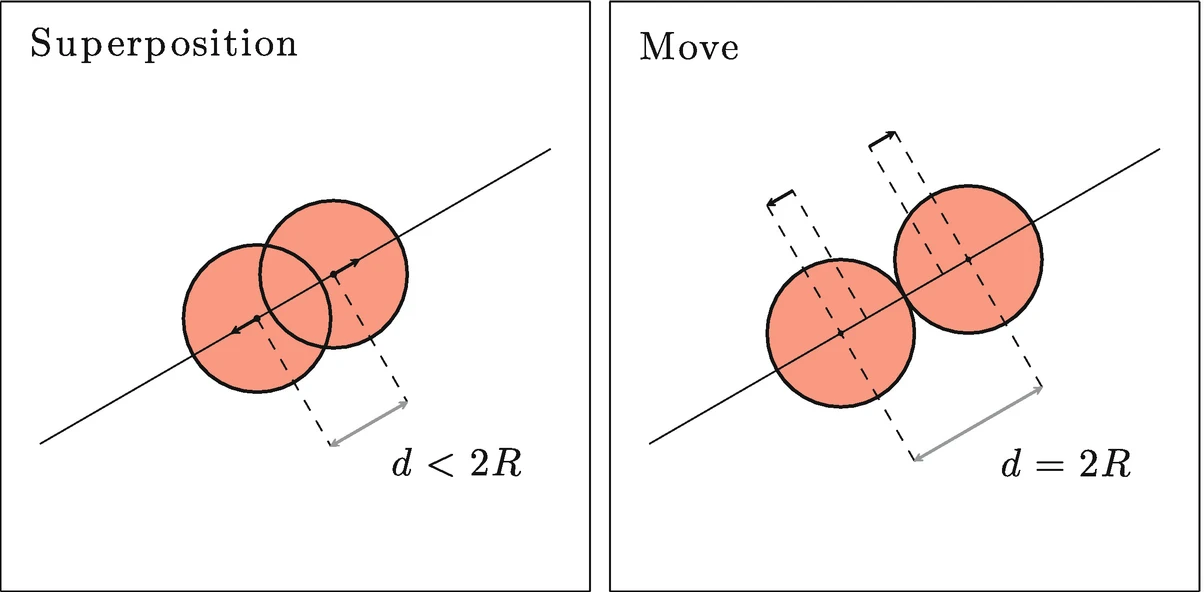
\includegraphics[width = 0.7\textwidth]{callegari_volpe_2019_hardsphere.png}
			\label{fig:hardsphere}
			\caption{ \cite{callegari_numerical_2019}}
		\end{figure}

	This operation involves calculating the distance matrix of a set of $n$ particles, i.e.~computing $n^2$ distances. Being a $O(n^2)$ algorithm, this kind of correction can become computationally demanding, especially for high density and velocity systems, where collisions and clustering are more likely to happen. Moreover, the one showed in algorithm \ref{alg:hardsphere} is just one step: there is no guarantee that after moving all particles every superposition will be removed. It becomes important to let the algorithm have a small tolerance, like $1/1000$ of particle radius and to cycle the correction until the number of superposition becomes $0$.
	
	Some works, such as \cite{martin-gomez_collective_2018, caprini_spontaneous_2020} use some kind of very steep repulsive potential ($\sim r^{-12}$) in order to simulate the excluded volume. In principle, since it does not require cycling, this approach seems faster, especially if one has to compute interactions anyway like in our case. During the development of this thesis some tests were run and, with all integration algorithms, even though computing the excluded volume effect is actually faster than applying a hard sphere correction, the steep potentials involved require a much smaller time step (1 or 2 orders of magnitude) which, in the end, makes simulating a fixed time lapse of dynamics slower.
	
	Since hard sphere corrections were implemented to study ABPs in confinement rather than open periodic boundary, this interaction could not take periodicity into account leading to possible superpositions at the simulation box borders.
	
	Finally, let us explain the physics behind this kind of correction. Moving superimposing particles of just the right amount to keep them in contact may seem a somehow strong assumption, since it is simulating a perfectly inelastic collision. Actually, if one wanted to simulate balls moving on a pool table, where macroscopic Newtonian dynamics take place, it would be easy to state whether collisions are elastic or not (in the mentioned case, yes). Here we can exploit what was found by, among others \citeauthor{singh_pair_2024} in \cite{singh_pair_2024}, where the contact time for Janus colloids was characterized, in different collision scenarios. They found contact times of the order of $\sim \text{s}$, similarly to what is often observed in Microscale Robotics Lab, motivating the choice of a completely inelastic collision, where adhesion forces keep particles together after the impact. 

	\section{Periodic Steric Interactions}
	When boundary conditions are periodic, not taking them into account in steric interactions may cause some problems, on top of being not formally correct. With the hard sphere correction as it was described before, particles are moved only when their distance is less than a diameter. As explained before, with periodic boundary conditions, a particles is reflected e.g.~on the left side only when its center of mass is out of the right border of more than a radius, meaning the particle must be entirely out before being reflected. If not taken into account, this may leave a \emph{frame} of size R around the box where particles can superimpose. 
	
	In the new version of this correction, distances are not computed in a Euclidean fashion anymore, but x and y components are separately checked, taking $\Delta x = min \left\{ \abs{x_1-x_2}, \abs{x_1-x_2}-L \right\}$, and the same for $y$, where $L$ is the box size. If one of the two particles is coming out of the box, but it has not been reflected yet, and the other is at the boundary, their difference in one component is larger than $L$. This way it is possible to identify superpositions at the borders, giving the possibility to form cluster starting from a \emph{nucleation site} on the boundary. 
	
	Another, more serious consequence is that, when working with potentials that feature a \emph{soft} non-superposition condition, like a diverging positive force at a $2R$ distance, two particles sticking out of the border on opposite sides may superimpose a lot before one of them gets reflected on the other side, but when this happens, the force between them diverges, leading to instabilities in the simulation.
	
	\section{All to All Central Potentials}
	Spring, Coulomb, Lennard Jones, Yukawa, Weeks-Chandler-Anderson are just few examples of the myriad of central potentials that are used to model interactions in physics. The central potential is the basis of this thesis too, and having a fast implementation is crucial to simulate interactions in large systems of particles. 
	
	The first step is to compute a distance matrix between the coordinates of all particles. Then a function $F(r)$ is applied to all the entries of this matrix to get the magnitude of the force between each pair of particles. We are simulating in 2D, so one way to get the radial direction for the force is to compute distance matrices both for $x$ and $y$ coordinates and then dividing them by the Euclidean distance matrix element-wise to get sine and cosine of the radial directions angle. Now the force is split in its two components and it can simply be added to the deterministic step in the coordinate as in algorithm \ref{alg:sim1}, given that we are in low Reynolds number regime. 
	
	\section{Interactions Range}
	In some situations is useful to have a way to restrict the force computation only to particles closer than a threshold distance.
	
	One could do this to imitate a topological interaction at short range, where a particle only interacts with its nearest neighbors. In the case of circular particles (or spherical in 3D), setting the range to $3R$ is enough to get this effect, since two particles in contact will have their centers at $2R$ and no other particle can be at less than $3R$ in the same directions. This way, central particle will interact with 6 other particles at most (this is the number of nearest neighbors for circular particles in 2D) giving the effect of a nearest neighbor interaction in the case of contact. Clearly, this is not a \emph{true} topological interaction, where two nearest neighbors interact regardless their distance, but it can give similar effects if applied in high packing fraction cases, where particles come in contact.
	
	Moreover, when dealing with fast decreasing potentials, it is possible for the magnitude of the force between two particles to be less than the machine epsilon. If this is the case, it is obviously pointless to look into pairs of particles which are more than a certain distance apart. One can compute this distance for any given potential, provided some reference magnitude. An example is given in Figure \ref{fig:force_zero}.
	\begin{figure}[htp]
		\centering
		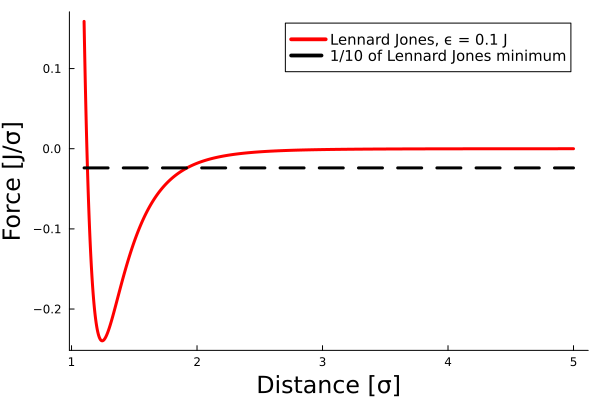
\includegraphics[width=\textwidth]{lj_zero.png}
		\caption{Cutoff for Lennard Jones force at $1/10$ of the minimum. The cutoff distance is $1.9\sigma$}
		\label{fig:force_zero}
	\end{figure}
	This is of paramount importance for speed. While a complete calculation of all the possible forces between $n$ particles is an $\order{n^2}$ algorithm (the actual number of possible interactions is $n(n-1)$), the number of particles in a box of given area is constant in $n$ if density remains fixed, so, scaling up the number of particles in the same conditions will be less demanding in terms of computational power.
	
	Inserting a range in interactions makes straightforward to apply them in a periodic fashion. Original code had a function to reflect particles in periodic boundary conditions, which worked in a very fast vectorized way (pseudo code for naive version is in algorithm \ref{alg:pbc}). The idea is: take one particle and make it the \emph{central} one, then shift coordinates of the other particles so that the \emph{central} is in $(0,0)$, now just apply periodic boundary conditions to the shifted coordinates. This process should guarantee that the \emph{central} particle interacts only once with any of the others, following a simple rule: when choosing between the true particle and the periodically shifted one the interacting particle is the closest one. An explanation of this process can be found in Figure \ref{fig:periodicint}.
	
	\begin{figure}[htp]
		\centering
		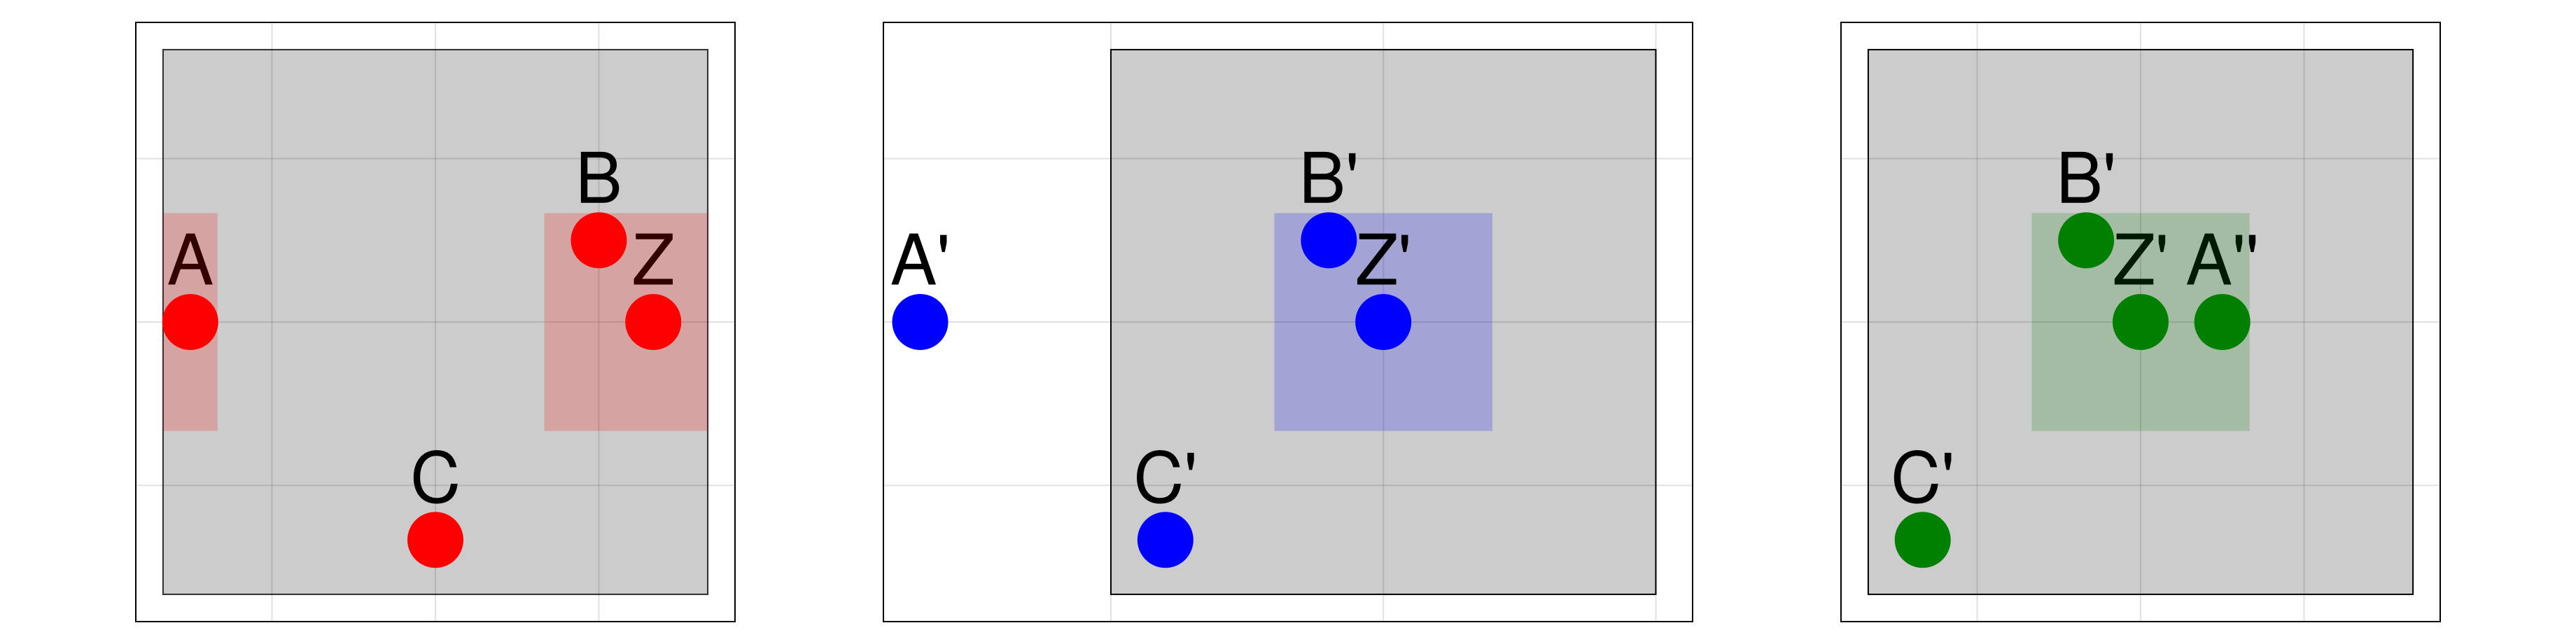
\includegraphics[width=\textwidth]{periodic_interaction.png}
		\caption{Red: original points with Z as central point and its interaction box sticking out on the opposite side. Blue: shifted points (blue) w.r.t.\ Z, Green: shifted points with PBC applied.}
		\label{fig:periodicint}
	\end{figure}
	
	\section{Aligning Interactions}
	

\end{document}